Lo primero que comprobamos del dataset es su gran tamaño, hay un total de 296021 muestras con 208 atributos cada una. Por lo que queda claro que vamos a proceder a reducir el dataset en la medida de lo posible.

Vamos a proceder a eliminar el atributo \textbf{appearedLocalTime}, la eliminamos en primer lugar por la dificultad de trabajar con este dado, el cual podríamos transformar en una serie de variables que desglosasen su contenido, no obstante tenemos otros atributos que ya lo hacen, como son la hora, el día, el mes y el año del avistamiento. Por otro lado vamos a eleminar también el atributo \textbf{X\_id} que como ya hemos comentado no sabemos qué representa. Además teniendo en cuenta que la aplicación se lanzó el día 6 de julio de 2016, es claro que no el año del avistamiento no aporta ninguna información, con lo que también eliminaremos el atributo \textbf{appearedYear}.

Viendo el dataset nos hemos dado cuenta de que para los atributos booleanos que nos indican si hay un gimnasio o una pokeparada a una distancia determinada del lugar de avistamiento del pokemon, siguen un patrón, y es que, al parecer, estas variables lo que indican es si hay un gimnasio o una pokeparada en un radio de una determinada longitud, con lo cual en cuanto el atributo que indica si hay un gimnasio a una distancia es cierto, el resto de atributos que indican si hay un gimnasio a una distancia mayor también lo son. 

Lo mismo sucede con las paradas. Entonces una vez hayamos confirmado esto, como la existencia de un gimnasio o una pokeparada en un radio determinado implica la existencia en un radio mayor, podremos eliminar, sin pérdida de información, todos estos atributos y quedarnos únicamente con los atributos \textbf{gymDistanceKm} y \textbf{pokestopDistanceKm}, que resumirían la información contenida en los otros atributos. Para tratar de comprobar esto vamos a hacer uso de las reglas de asociación con el paquete \textbf{arules}.

Hemos obtenido las distintas reglas de asociación sin atender al soporte ya que no estamos interesados en saber cuantas veces se da una correspondencia entre dos hechos (el soporte de dicha regla), lo que queremos saber es que cuando se da un hecho, esto implica que se den los que suponemos que deberian darse (la confianza de las reglas encontradas). 

Por tanto, como podemos ver, las reglas de asociación encontradas prueban nuestras suposiciones. Dado esto, procedemos a elminar los atributos. Como la confianza es del 100\%, no afecta haber usado el conjunto entero.

Este dataset nos proporciona una serie de atributos para la localización del pokemon. Los primeros que nos encontramos son latitude y longitude, se tratan de coordenadas geográficas. Por otro lado aparecen \textbf{cellId\_90m}, \textbf{cellId\_180m}, \textbf{cellId\_370m}, \textbf{cellId\_730m}, \textbf{cellId\_1460m}, \textbf{cellId\_2920m}, \textbf{cellId\_5850m}. 

Estos indican la posición geográfica usando celdas s2. Estas celdas se clasifican en niveles atendiendo a su área, desde 0 (menor área) a 30 (mayor área). Se obtienen según longitud y latitud, por lo que son la misma información representada de distinta manera. Además para métodos que dependen de una distancia como el KNN tendríamos que investigar la distancia entre las distintas celdas a través de su ID, lo que supondría una carga de trabajo extra e innecesaria. 

Se puede consultar más información sobre las celdas s2 en el siguiente \href{http://blog.christianperone.com/2015/08/googles-s2-geometry-on-the-sphere-cells-and-hilbert-curve/}{enlace}

Por lo comentando arriba se va a optar a eliminar los atributos correspondientes a las celdas, dejando los atributos latitude y longitude como los únicos para determinar la posición.

Una vez que hemos limpiado el dataset, vamos a añadir información que falta pero nos va a resultar útil de cara a realizar clasificación y asociación. 

Esta información son los tipos asociados a cada pokemon, pudiendo ser: agua, fuego, planta, hielo... y el nombre propio de cada pokemon.

Como ya hemos dicho en nuestro dataset tenemos información que nos permite conocer la posición en la que se produjo un avistamiento. Sin embargo, cuando pintamos los avistamientos que tenían como ciudad Madrid en el atributo city nos encontramos lo siguiente:

\begin{figure}[H] %con el [H] le obligamos a situar aquí la figura
\centering
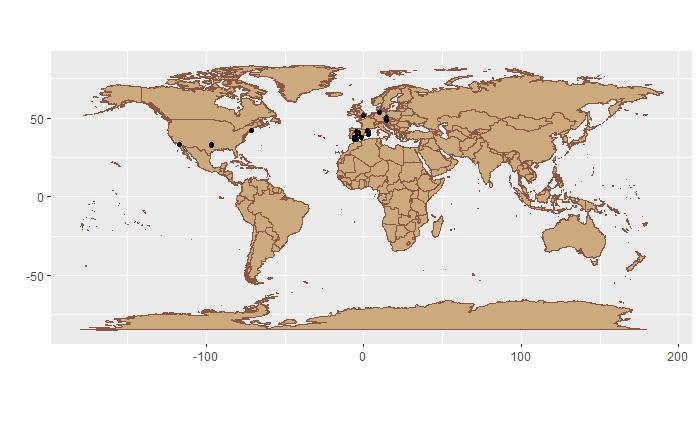
\includegraphics[scale=0.8]{img/madrid.jpg}  %el parámetro scale permite agrandar o achicar la imagen. En el nombre de archivo puede especificar directorios
\label{img/madrid.jpg}
\caption{Avistamientos Madrid}
\end{figure}

Es decir hay puntos en Madrid que no están situados en el mapa en una posición cercana a Madrid. En un principio pensamos que esto se debía a que el sistema de coordenadas del mapa sobre el que dibujamos los puntos, y los de la longitud y la latitud de nuestro dataset no coincidían. Pero antes decidimos dibujar los avistamientos relativos a pokemon que sólo aparecen en una regiones exclusivas: Mr. Mime en Europa, Tauros en Norte América, Kangaskhan en Australasia y Farfetch'd en Asia:

\begin{figure}[H] %con el [H] le obligamos a situar aquí la figura
\centering
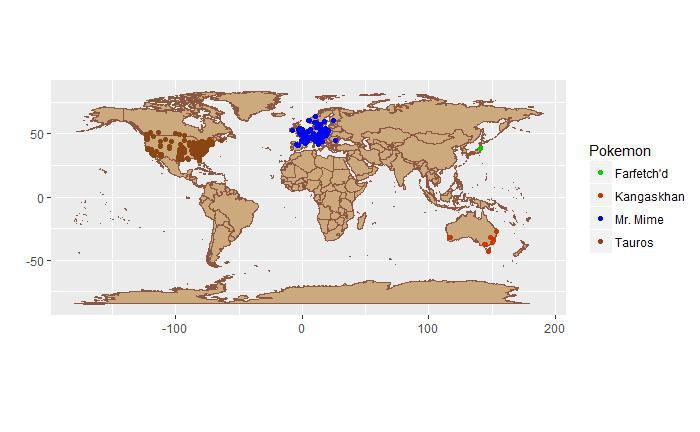
\includegraphics[scale=0.8]{img/exclusivos.jpg}  %el parámetro scale permite agrandar o achicar la imagen. En el nombre de archivo puede especificar directorios
\label{img/exclusivos.jpg}
\caption{Avistamientos regiones exclusivas}
\end{figure}

Como podemos ver la localización de estas visualizaciones es correcta, por lo tanto consideramos que las descripción del creador del dataset del atributo \textbf{city} no es correcta  \textbf\textit{the city of a sighting}. Así que o bien este atributo es la ciudad del usuario que vio el pokemon o el uso de proxys (que muchos usuarios emplearon para falsificar su posición y así poder acceder a pokemon de otras localizaciones distintas a la suya real) ha falseado los datos. En cualquiera de los casos esta información no es de utilidad para la predicción que queremos realizar con lo que la eliminaremos, junto con el atributo\textbf{continent}.

Pero antes vamos a emplear esta información. Y es que debemos pensar que un dataset no ha de servir únicamente para el problema que se plantea con él. Al tener datos de una aplicación empleada por tantos usuarios internacionalmente el número de datos indirectos que podemos extraer de él es muy grande, y de gran utilidad. En esta ocasión, considerando que el atributo \textbf{city} se refiere a la ciudad del usuario y que por tanto la localización de las observaciones se debe a viajes reales realizados por los usuarios, podemos extraer información sobre los desplazamientos realizados por los usuarios de la aplicación. En esta ocasión nos vamos a centrar en ver los viajes realizados por habitantes de Oslo:

\begin{figure}[H] %con el [H] le obligamos a situar aquí la figura
\centering
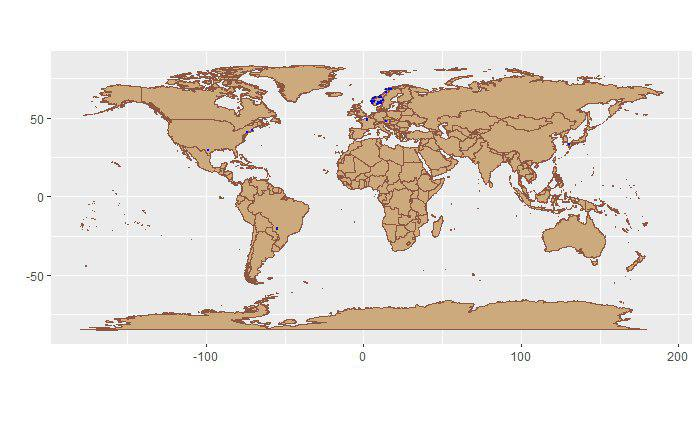
\includegraphics[scale=0.8]{img/oslo.jpg}  %el parámetro scale permite agrandar o achicar la imagen. En el nombre de archivo puede especificar directorios
\label{img/oslo.jpg}
\caption{Viajes realizados por los habitantes de Oslo}
\end{figure}

Como es natural, eliminamos \textbf{city}  

En relación a estos datos indirectos que podemos obtener a partir de nuestro dataset podemos obtener también un mapa de temperaturas en el que se muentren las temperaturas de los avistamientos. Como veremos más adelante los datos son relativos a una semana de agosto con lo que vamos a mostrar la temperatura referente a todos los avistamientos del dataset en un mismo mapa:

\begin{figure}[H] %con el [H] le obligamos a situar aquí la figura
\centering
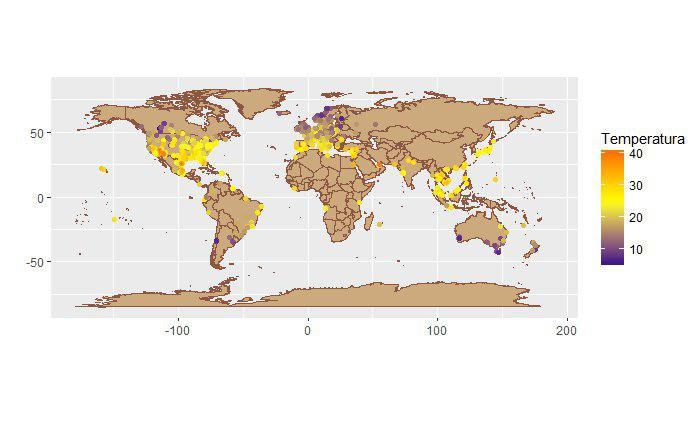
\includegraphics[scale=0.8]{img/temperatura.jpg}  %el parámetro scale permite agrandar o achicar la imagen. En el nombre de archivo puede especificar directorios
\label{img/temperatura.jpg}
\caption{Temperatura de los avistamientos}
\end{figure}

Aquí podemos apreciar por ejemplo con en Argentina las temperaturas son bajas en agosto, y como hay una diferencia de temperatura entre el norte y el sur de Europa.









